\documentclass{beamer}
\usepackage{graphicx}

% Set image search paths
\graphicspath{{../images/}{../../shared/images/}}

\usetheme{Madrid}
\usecolortheme{default}

% Define custom colors
\definecolor{ds9blue}{RGB}{25,25,112}
\definecolor{ds9gold}{RGB}{218,165,32}
\definecolor{ds9grey}{RGB}{105,105,105}
\definecolor{ds9red}{RGB}{178,34,34}

% Set theme colors
\setbeamercolor{structure}{fg=ds9blue}
\setbeamercolor{title}{fg=ds9blue,bg=ds9gold!20}
\setbeamercolor{frametitle}{fg=ds9blue,bg=ds9gold!10}
\setbeamercolor{block title}{fg=white,bg=ds9blue}
\setbeamercolor{block body}{fg=black,bg=ds9gold!10}

% Title page info
\title[Circular Motion]{PHYS12 CH6: Gravitation and Keplar's Laws}
\subtitle{Sections 6.5-6.6}
\author[Mr. Gullo]{Mr. Gullo}
\date[Feb 2025]{February, 2025}

\begin{document}

\frame{\titlepage}

\begin{frame}
\frametitle{Learning Objectives}
By the end of this lesson, you will be able to:
\begin{itemize}
  \item Understand and explain Earth's gravitational force
        \item Describe the mathematical form of Newton's Universal Law of Gravitation
        \item Calculate gravitational forces between masses
        \item Explain the significance of the gravitational constant G
        \item Discuss the historical development of gravitational theory
\end{itemize}
\end{frame}

\begin{frame}{Historical Development}
    \begin{columns}
        \column{0.5\textwidth}
        \begin{itemize}
            \item Newton (1687): First precise definition of gravitational force
            \item Showed it explains both:
                \begin{itemize}
                    \item Falling objects on Earth
                    \item Astronomical motions
                \end{itemize}
            \item du Châtelet's contributions:
                \begin{itemize}
                    \item Translation and augmentation
                    \item Use of calculus to explain gravity
                \end{itemize}
        \end{itemize}
        \column{0.5\textwidth}
        
        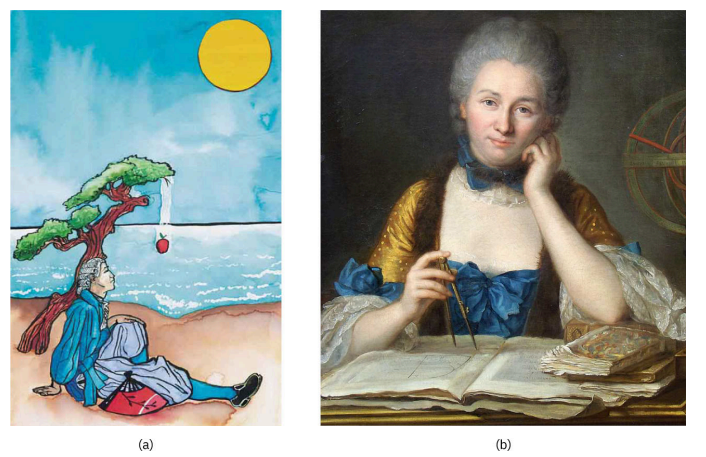
\includegraphics[width=\textwidth]{phys12-gravity-newtons-cannon-thought-experiment.png}

        \end{columns}
\end{frame}

\begin{frame}
\frametitle{Video Media}
\begin{itemize}
 \item https://www.youtube.com/watch?v=7gf6YpdvtE0
\end{itemize}
\end{frame}

\begin{frame}
\frametitle{Newton's Universal Law of Gravitation}
\begin{itemize}
    \item Every particle in the universe attracts every other particle with a force along a line joining them
    \item Force is:
        \[ F = G\frac{m_1m_2}{r^2} \]
    where:
    \begin{itemize}
        \item $G = 6.674 \times 10^{-11}$ N$\cdot$m$^2$/kg$^2$
        \item $m_1, m_2$ are the masses of the objects
        \item $r$ is the distance between their centers
    \end{itemize}
    \item The force is always attractive
    \item It follows the inverse square law
\end{itemize}
\end{frame}

\begin{frame}
\frametitle{Gravity and Circular Motion}
\begin{itemize}
    \item For objects in circular orbit:
        \[ F_g = F_c \]
    \item This means:
        \[ G\frac{mM}{r^2} = m\frac{v^2}{r} \]
    \item Solving for orbital velocity:
        \[ v = \sqrt{\frac{GM}{r}} \]
    \item Applications:
    \begin{itemize}
        \item Planetary orbits
        \item Artificial satellites
        \item Space stations
    \end{itemize}
\end{itemize}
\end{frame}

\begin{frame}{The Cavendish Experiment}
    \begin{columns}
        \column{0.6\textwidth}
        \begin{itemize}
            \item First accurate measurement of G (1798)
            \item Measured tiny gravitational attraction between lead spheres
            \item Led to first calculation of Earth's mass
            \item Modern version still used today
        \end{itemize}
        \column{0.4\textwidth}
        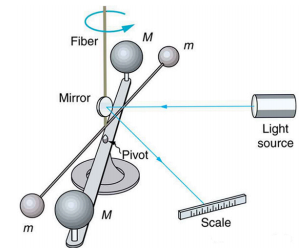
\includegraphics[width=\textwidth]{phys12-gravity-cavendish-experiment.png}
    \end{columns}
\end{frame}

\begin{frame}{Example: Earth's Gravitational Force}
    \begin{block}{Problem}
        Calculate the gravitational force between Earth ($M = 5.97 \times 10^{24}$ kg) and a 70 kg person at Earth's surface ($R = 6.37 \times 10^6$ m).
    \end{block}
    \begin{solution}
        \begin{align*}
            F &= G\frac{Mm}{r^2} \\
            &= (6.67 \times 10^{-11})\frac{(5.97 \times 10^{24})(70)}{(6.37 \times 10^6)^2} \\
            &= ??? \text{ N}
        \end{align*}
    \end{solution}
\end{frame}



\begin{frame}
\frametitle{Kepler's First Law: Elliptical Orbits}

\textbf{Statement:}
\begin{itemize}
    \item All planets orbit the Sun in elliptical paths
    \item The Sun is located at one focus of the ellipse
\end{itemize}

\textbf{Properties of Elliptical Orbits:}
\begin{itemize}
    \item \textbf{Semi-major axis} ($a$): half the longest diameter
    \item \textbf{Eccentricity} ($e$): measures deviation from circular orbit
    \begin{itemize}
        \item $e = 0$: perfect circle
        \item $0 < e < 1$: ellipse
        \item Most planetary orbits have small $e$
    \end{itemize}
    \item \textbf{Perihelion}: closest approach to Sun
    \item \textbf{Aphelion}: farthest point from Sun
\end{itemize}

\textbf{Implications:}
\begin{itemize}
    \item Distance from Sun varies during orbit
    \item Orbital speed varies (connects to Second Law)
    \item True for all orbiting bodies under gravity
\end{itemize}

\end{frame}

\begin{frame}
\frametitle{Video Media}
\begin{itemize}
 \item https://www.youtube.com/watch?v=Dvoe8Ib5D1o
\end{itemize}
\end{frame}

\begin{frame}
\begin{figure}
    \centering
    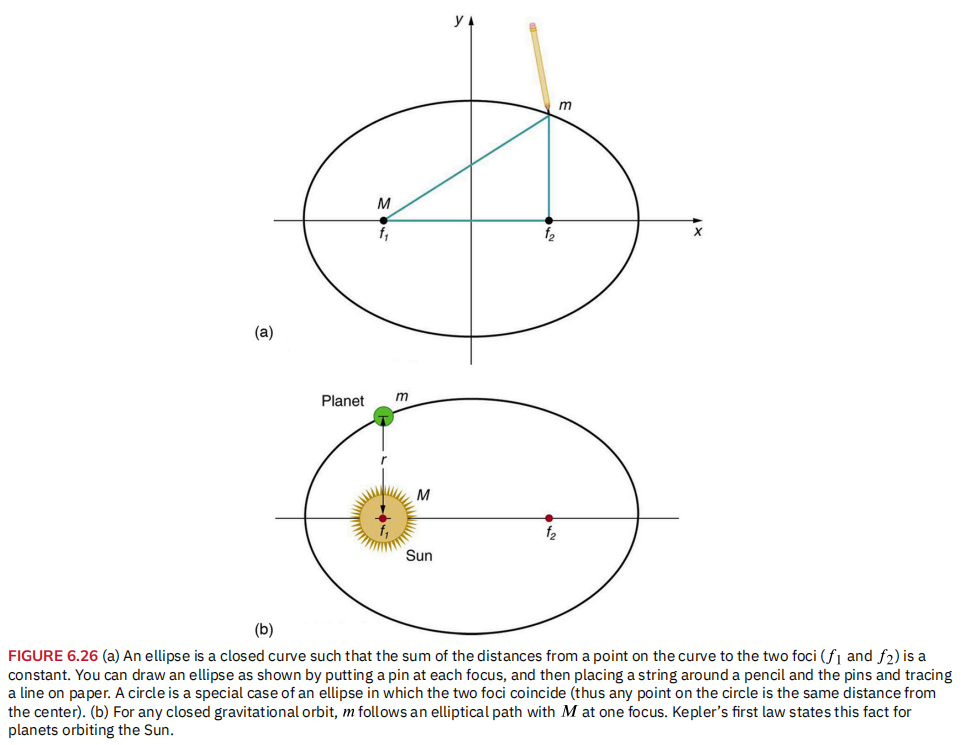
\includegraphics[width=1\linewidth]{phys12-gravity-keplers-first-law.png}
\end{figure}
\end{frame}

\begin{frame}
\frametitle{Kepler's Laws: Equal Areas (Second Law)}
\begin{columns}
\begin{column}{0.6\textwidth}
\textbf{Kepler's Second Law:}
\begin{itemize}
    \item A line from the Sun to a planet sweeps out equal areas in equal times
    \item The shaded regions ($A_1$, $A_2$, $A_3$) have equal areas
    \item Important implications:
    \begin{itemize}
        \item Planet moves fastest when closest to Sun
        \item Planet moves slowest when farthest from Sun
        \item Angular momentum is conserved
    \end{itemize}
\end{itemize}
\end{column}
\begin{column}{0.4\textwidth}

\end{column}
\end{columns}
\end{frame}

\begin{frame}
\begin{figure}
    \centering
    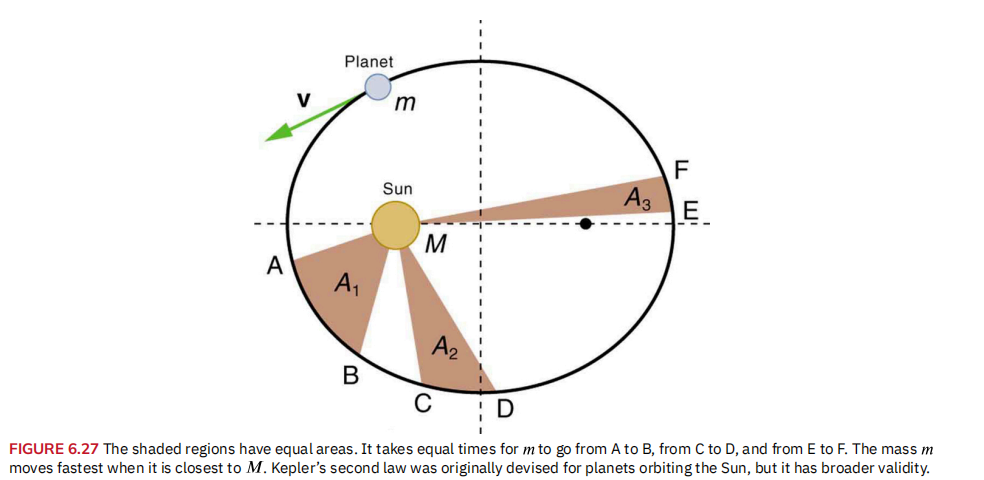
\includegraphics[width=1\linewidth]{phys12-gravity-kepler-orbital-diagram.png}
\end{figure}
\end{frame}

\begin{frame}
\frametitle{Kepler's Third Law of Planetary Motion}

\textbf{Mathematical Statement:}
\[ \frac{T_1^2}{T_2^2} = \frac{r_1^3}{r_2^3} \]
where:
\begin{itemize}
    \item $T$ = orbital period
    \item $r$ = average orbital radius
    \item Subscripts 1,2 refer to different planets
\end{itemize}

\textbf{Key Points:}
\begin{itemize}
    \item Relates orbital period to orbital radius
    \item Squared period proportional to cubed radius
    \item Valid for all objects orbiting same central mass
    \item Can be derived from Newton's laws and universal gravitation
\end{itemize}

\textbf{Example:}
If Planet 1 has period 1 year at 1 AU, a planet at 4 AU would have period:
\[ T_2 = \sqrt{4^3} = 8 \text{ years} \]
\end{frame}


\begin{frame}
\begin{figure}
    \centering
    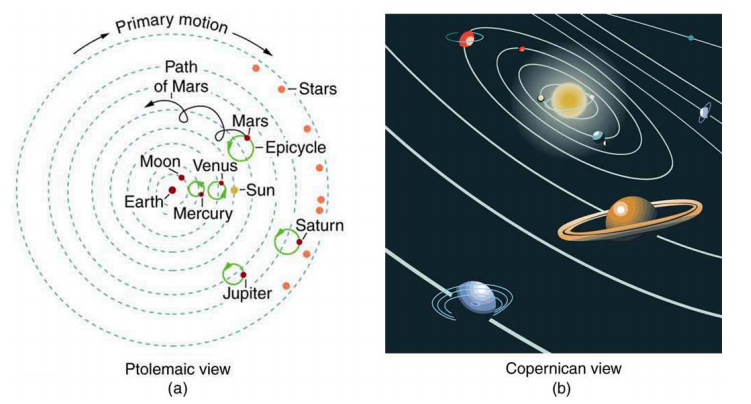
\includegraphics[width=1\linewidth]{phys12-circuits-circuit-model-views.png}
\end{figure}
\end{frame}


\begin{frame}
\frametitle{Video Media}
\begin{itemize}
  \item https://www.youtube.com/watch?v=yC74lhJX9Ck
\end{itemize}
\end{frame}


\begin{frame}
\frametitle{What is a Planet? IAU Definition (2006)}

\begin{block}{Official IAU Definition}
A planet in our solar system is a celestial body that:
\end{block}

\begin{enumerate}
    \item Is in orbit around the Sun
    \begin{itemize}
        \item Regular, elliptical orbit
        \item Primary gravitational relationship with Sun
    \end{itemize}
    
    \item Has sufficient mass for hydrostatic equilibrium
    \begin{itemize}
        \item Strong enough gravity to become spherical
        \item Overcomes rigid body forces
    \end{itemize}
    
    \item Has cleared its orbital neighborhood
    \begin{itemize}
        \item Gravitationally dominant in its orbit
        \item No similar-sized objects in its orbital path
    \end{itemize}
\end{enumerate}
\end{frame}

\begin{frame}
\frametitle{Dwarf Planets and the Case of Pluto}

\begin{block}{Dwarf Planet Definition}
A celestial body that:
\begin{itemize}
    \item Orbits the Sun
    \item Has hydrostatic equilibrium
    \item Has NOT cleared its orbital neighborhood
\end{itemize}
\end{block}

\begin{itemize}
    \item Pluto was reclassified in 2006
    \item Reasons for reclassification:
    \begin{itemize}
        \item Shares its orbit with many Kuiper Belt objects
        \item Not gravitationally dominant in its region
        \item Similar to other objects in its orbital zone
    \end{itemize}
    \item Other recognized dwarf planets:
    \begin{itemize}
        \item Ceres (in asteroid belt)
        \item Eris (beyond Pluto)
        \item Haumea and Makemake (Kuiper Belt)
    \end{itemize}
\end{itemize}

\end{frame}
\begin{frame}
\begin{figure}
    \centering
    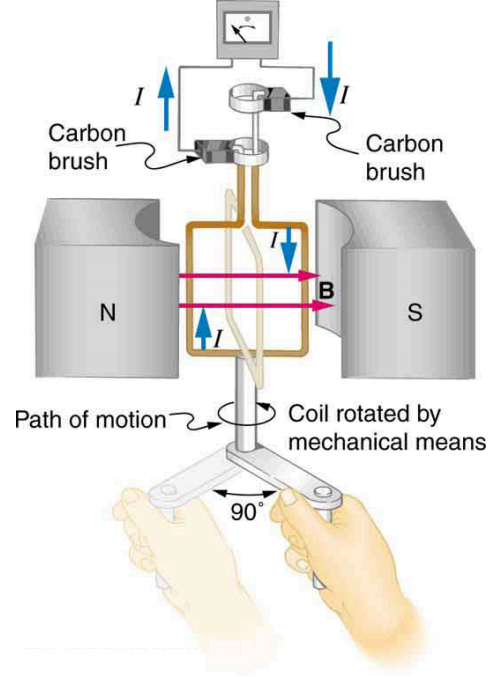
\includegraphics[width=1\linewidth]{phys12-circuits-rc-circuit-diagram.png}
\end{figure}
\end{frame}

\begin{frame}
\frametitle{Summary}
\textbf{Universal Gravitation:}
\begin{itemize}
    \item \textbf{Newton's Law:} $F_g = G\frac{m_1m_2}{r^2}$
    \item \textbf{Gravitational Constant:} $G = 6.674 \times 10^{-11}$ N$\cdot$m$^2$/kg$^2$
    \item \textbf{Historical Development:} Newton's theory and du Châtelet's contributions
    \item \textbf{Cavendish Experiment:} First measurement of G
\end{itemize}

\textbf{Kepler's Laws:}
\begin{itemize}
    \item \textbf{First Law:} Planets follow elliptical orbits with Sun at one focus
    \item \textbf{Second Law:} Equal areas in equal times
    \item \textbf{Third Law:} $\frac{T_1^2}{T_2^2} = \frac{r_1^3}{r_2^3}$
\end{itemize}

\textbf{Orbital Motion:}
\begin{itemize}
    \item \textbf{Orbital Velocity:} $v = \sqrt{\frac{GM}{r}}$
    \item \textbf{Gravitational Force = Centripetal Force:} $F_g = F_c$
    \item \textbf{Applications:} Planets, satellites, space stations, astroid mining
\end{itemize}
\end{frame}

\end{document}